\documentclass[10pt]{article}
\usepackage[text={6in,8.1in},centering]{geometry}
\usepackage{enumerate}
\usepackage{amsmath,amsthm,amssymb}
\usepackage{mathrsfs} % to use mathscr fonts
\newcommand{\mcL}{\mathcal{L}}
\newcommand{\mcI}{\mathcal{I}}
\newcommand{\mcM}{\mathcal{M}}
\newcommand{\mcP}{\mathcal{P}}
\newcommand{\mcX}{\mathcal{X}}
\newcommand{\mcK}{\mathcal{K}}
\newcommand{\mcG}{\mathcal{G}}
\newcommand{\mcC}{\mathcal{C}}
\newcommand{\mcS}{\mathcal{S}}
\newcommand{\mcD}{\mathcal{D}}
\newcommand\ninepointscircle[3]{}
\usepackage{tikz}
\usetikzlibrary{calc,through,intersections}
\usepackage{ifthen}
\usepackage{geometry}
\DeclareMathOperator*{\argmax}{arg\,max}
\DeclareMathOperator*{\argmin}{arg\,min}
\newenvironment{block}{\begin{adjustwidth}{1.5cm}{1.5cm}\noindent}{\end{adjustwidth}}
\newtheorem{proposition}{Proposition}[section]
\newtheorem{theorem}{Theorem}[section]
\newtheorem{lemma}{Lemma}[section]
\newtheorem{corollary}{Corollary}[section]
\theoremstyle{definition}
\newtheorem{definition}{Definition}[section]

\begin{document}

\section{Proposed Topic}

In order to construct a
viable model of a game, we must have (1) self-configuration, and (2) automatic neighbor
relations. We address our players as a finite set of actions, and attempt to formalize the game play as sphere-of-
influence (SIG) graph. To begin, we propose a set of mixed strategies defined by a probability
distribution over the finite set of feasible strategies, and define a basic game
played by intelligent players.
We make use of mean field theorem to prove the existence of a dense strategy
space, and define a decision model in the
extended (compacted) strategy space determined by a drift diffusion process.

Given a stochastic arrival process, we define a subset of the field of
right-continuous, left-limited \emph{cadlag} 
functions, and show there exists a mapping of player types to a time-dependent
arrangement, where we may then apply our statistical game theoretic approach.
We conjecture that the choice of arrangement and random process results in a
proximity/incidence graph with nice properties.


\section{Proposed Theorem}

Let $\pi$ be a normalizing function acting on an angle $\theta \in \mathbb{C}$. 
The mapping $\mathbb{N} \mapsto \mcK\times \mcS$ exists if and only if there is
the product space $\lbrace \pi k \mapsto r(\tau)\rbrace$, where $k=1$ defines
the mapping 
$$
    \theta(\cdot, k) \mapsto \mcP^k \times \mcK.
$$
$\mcK$ is the space of \emph{cadlag} functions restricted to
$\mathbb{A}^\mathbb{R} \times [0,1]^\mathbb{R}$,
and $\mcP$ is the projective space of the
player's strategy distribution $\mcS$. We define right-continuity as 
a \emph{stopping time} $\tau:\mcS \rightarrow [0,+\infty]^\mathbb{R}$.

Let $\mcI$ be an arrangement on $\mcK$ where
$\theta (s_1, r(t)) > \theta (s_1, r(t+1))$ implies that $\pi k < \pi
(k+1)$ for all $t\in\tau$.
Then, fixing $t\in \tau$, let $\theta' \ne \theta$ be given by 
$$
    \theta' = \theta \cdot \displaystyle\sqrt{\frac{1+\beta^2}{1-\beta^2}},
$$
where $\beta = \tan\theta$. 

We claim that there exists a geodesic such that there is a
mapping from the origin, $0_{\mcS}$, is defined by the ball
$$
    B(\tau, \cdot) = \lbrace \lbrack s_i, s_{-i}\rbrack : i \in \mcI \subset
    \mcK\times \tau \rbrace,
$$
where $\lbrack \cdot, \cdot\rbrack : \mcS \times \mcS \mapsto \mcS$ is the Lie
bracket operator.

Suppose that $[s_i, s_{-i}] < 0_{\mcS}$. We have a cone projection in $\mcS_\tau$ 
\begin{center}
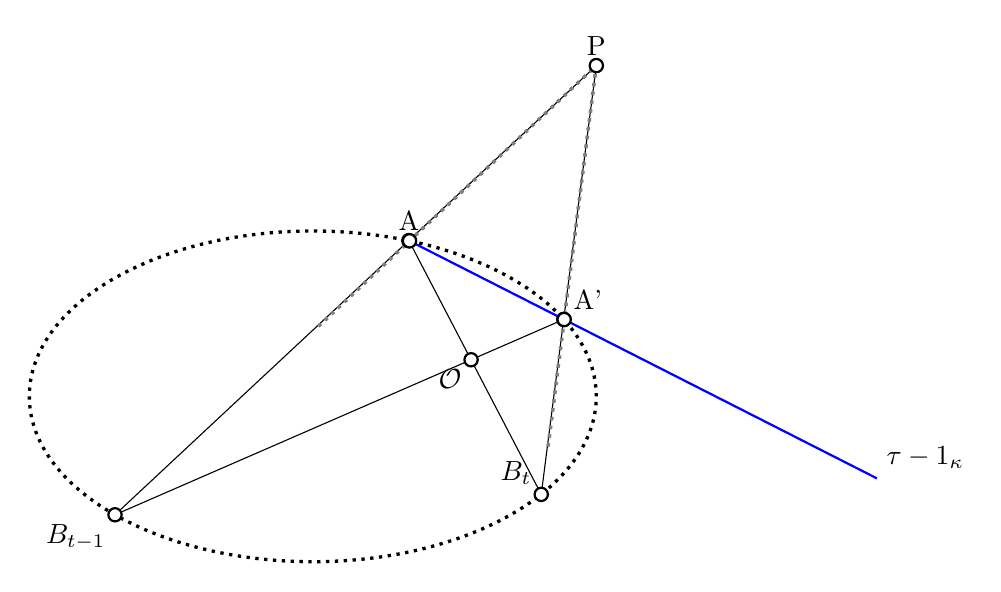
\begin{tikzpicture}[scale=1.2]
	\tikzset{mypoints/.style={fill=white,draw=black,thick}}
	\def\ptsize{2.0pt}
	\def\a{3} \def\b{1.75}
	% warning: construction fails if xp<0 or yp<=0
	\def\xp{3.0} \def\yp{3.5} 
	\def\i{0.85} \def\j{-0.25}%determines rays from P
	\coordinate[label=above:P] (P) at (\xp,\yp);
	\coordinate (M) at ({\a*\i},0);
	\coordinate (N) at ({\a*\j},0);
	\coordinate (AA) at (0,-\b);
	\coordinate (BB) at (1,-\b);
	\coordinate (CC) at (-\a,0);
	\coordinate (DD) at (-\a,1);
	\coordinate (Q) at (intersection of P--N and AA--BB);
	\coordinate (R) at (intersection of P--M and AA--BB);
	\draw[name path=ellipse,dotted,very thick]
		(0,0) circle[x radius = \a cm, y radius = \b cm];
	\path[name path=linePQ,blue] (P)--(Q);
	\path[name path=linePR,dotted] (P)--(R);
	\path [name intersections={of = ellipse and linePQ}];
	\coordinate[label=above:A] (A)  at (intersection-1);
	\coordinate[label=below left:$B_{t-1}$] (B) at (intersection-2);
	\path [name intersections={of = ellipse and linePR}];
	\coordinate[label=above right:A'] (C)  at (intersection-1);
	\coordinate[label=above left:$B_t$] (D) at (intersection-2);
	\draw (B)--(P)--(D) (A)--(D) (C)--(B);
	\coordinate [label=below left:$\mathcal O$] (E) at (intersection of A--D and B--C);
    \coordinate[label=above right:$\tau-1_\kappa$] (F) at (intersection of A--C and B--D);
	\draw [name path=lineFA,blue,thick] (F)--(A);
	\path [name intersections={of = ellipse and lineFA}];
	\coordinate[label=above:] (X) at (intersection-1);
	\coordinate[label=above right:] (Y) at (intersection-2);
	\coordinate (XX) at ($(P)!1.5!(X)$);
	\coordinate (YY) at ($(P)!1.5!(Y)$);
	\draw[very thick,dotted,black!50] (XX)--(P)--(YY);
	\draw[very thick,dotted,black!50,shift={(1:2)}] (XX)--(P)--(YY);
	\foreach \p in {A,B,C,D,E,P,X,Y}
		\fill[mypoints] (\p) circle (\ptsize);
  \end{tikzpicture}
\end{center}
We have a bijection from $\pi\mcK \in \mcS \times \mcS$ to $r(\tau) \in \mcS$
such that
$B_{s_{-i}}(\tau) < \pi\mcK$ reveals a sub-algebra extending the strategy space
with respect to the real variable $\tau$, and is a homeomorphy with respect to
the ... blah... and the expectation $\mathbb{E}[r(\tau)]$. %2 tau^K 
Thus, the resulting subspace topology is simply connected.

We claim that if $s$ is in the null space of the ball, then there exists an identity
operator such that $\pi\kappa(s) \mapsto [s]$.
Now, given a function $\phi$, we examine the
extended strategy space where $s_1$ stochastically dominating $s_2$ implies that
$\mathbb{E}[\phi (\cdot, s_2 )] > \mathbb{E}[\phi (\cdot, s_1 )]$. Suppose
$\phi^{-1}$ preserves the quadratic form $(t^2- \langle s \rangle) \mapsto (t, r, \theta)$, so
that
$$
    \displaystyle \int_t^{t+1} \phi^{-1}(\theta(\mcK)) dt = \theta(\cdot,
    k+1)-\theta(\cdot,k).
$$
We have that $2 \pi \delta \mcK \le \delta \mcS$?

The players arrive to the game at a rate determined by arrival process $\phi(\tau, \cdot)$. 
$$
    d\mcS_t = \theta(\cdot, t) \phi(\mcS_t) dt + \phi_t(\mcS_t) dW_t,
$$
where $W_t: [0, +\infty) \times \mcS \rightarrow \mcS$ is a one-dimensional
stop-time Brownian motion. 
As any cadlag finite variation process has quadratic variation equal to the sum
of the squares of the jumps $0=s_0<s_1<\cdots s_n$, the solution to
$$
    s_i(\tau) = \int_{\theta_i(s_i, t)}^{\theta_i(s_i,t+1)} \pi(\tau) \ d\tau
$$ 
for $t \in \tau$ gives a set of unique jumping points $0=s_0<s_1< \cdots < s_{\overline \mcK} = s_{MAX}$. 
Let each player's stop time $\tau$ occur at a random jumping point within their
strategy space, thereby fixing $\overline{\mcK}$ for that player.

We consider a ball $B$, where a nonzero flux at the boundary represents an
uncertainty state, and take a random measure on $(\mcS \times \mcS, \mcK)$, i.e.
the $\sigma(\phi)$-algebra of the arrival process.
Each ball $B$ represents a distribution of possible strategies, and as subset of the
measure space we are able to compute its density function. 
Define the density operator $\rho$ on $\mcS\times \mcS$ as
$$
    \rho = \displaystyle\sum \vert s_i\rangle\langle s_{-i}\vert
$$
where $\vert s_i\rangle\langle s_{-i}\vert$ is the outer product. The state
$[s]$ is an algebra of $\mcS\times\mcS$, with expectation
value given by $\langle [s] \rangle = \text{tr}{\rho [s]}$, and is pure imaginary.
We have that $2 \pi (\text{tr} \mcK - \text{tr} \rho S|_r) \le \delta \mcS$?
The density matrix used here is defined to be the statistical state of a system in
quantum mechanics, and is particularly useful in dealing with mixed states.
Define a graph $\mcG$ as the set subsets of $\mcS\times\mcS$ of fully connected nodes.
We claim that there exists an additional, induced metric, on $\mcG$.
The closed sphere of influence graph covers the intersections
of the closed balls $\lbrace\overline{B}\rbrace \subset \mcS\times \mcS$, where
$$
    \overline{B}= \lbrace B_i \in \mcS : \min\rho(s_i, s_{-i}) \le
    r_{\tau\times\tau} \rbrace.
$$
We finally claim to have an immersion in the surrounding
dynamical complex field $\mathbb{C}^{\tau\times\tau}$. The density matrix compresses
the space $\mcS \times \mcS$ to its canonical form. Thus, by Schur's lemma, the intertwining map
$phi^{-1} \mapsto S times S$, is either $0$, or an isomorphism.
Thus,$\mcG$ is a unitary structure that can be seen as an orthogonal structure, a complex
structure, and a symplectic structure.

TODO: FINISH!
The complex field $\mathbb{C}^{\tau\times\tau}$ encases the distributions of the
player strategies; that is, the gradient of the distribution across the boundary
of $\mcG$ determines the orientation of exterior. 
We proceed to determine the skew-distribution of the closed manifold. 
We examine the skew-Hermetian assignment, and the resulting tangent vector, or four-velocity. 
The four coordinate functions $\theta^c (\tau), c = 0, 1, 2, 3$ are real
functions of a real variable $\tau$. 
We have that $\phi\cdot \mcS\subset \mcS$ is the subset of skew-Hermetian matrices known as signed
permutation matrices. We extend our mean-field model to include this
representation by setting $\begin{bmatrix}0 \\ k\end{bmatrix} = \begin{bmatrix}1
\\ k\end{bmatrix}$ at the stop time $\tau$. 

Define the the player's initial utility
function as a hyperbolic absolute risk aversion (HARA), and so must adhere to,
for utility $\mu$,
$$
    \displaystyle\frac{\mu''(\langle s_i,s_{-i}\rangle)}{\mu'(\langle s_i,
    s_{-i})}.
$$

\section{Research Plan}

\begin{itemize}
	\item Step 1: Formulate the relevant graph models using appropriate abstraction.
	\item Step 2: Establish the existence/uniqueness of differential tensor/flow .
	\item Step 3: Implement a python/ruby module/scaffolding to model to aid in prototyping
    conditions to define (possible) deterministic systems. 
	\item Step 4: Based on the analytical results, implement various systems' tensorflow.
\end{itemize}

\section{References}

$[1]$ "Sphere of Influence Graphs in General Metric Spaces", T.S. Michael, T. Quint\\
$[2]$ "The Supermarket Game", Jiaming Xu, Bruce Hajek\\
$[3]$ "Self-coexistence among interference-aware IEEE 802.22 networks with enhanced air-interface", S. Sengupta, S. Brahma, M. Chatterjee, N. Sai Shankar\\

\section{Literature}

In addition to related work, the sourced literature must include historical
papers to give perspective and formalization, and determine the foundation of
the proposed theory.\\
$[1]$ M. E. Bratman. Intention, Plans, and Practical Reason. CSLI Publications, Stanford University,
1987.\\
$[2]$ I. Gilboa and E. Zemel. Nash and correlated equilibria: Some complexity considerations. Games
and Economic Behavior, 1:80-93, 1989.\\
$[3]$ E. Kalai. Games, computers, and O.R. In ACM/SIAM Symposium on Discrete Algorithms, 1995.\\
$[4]$ Noam Nisan and Amir Ronen. Algorithmic mechanism design. In Proc. 31st ACM Symp. on
Theory of Computing, pages 129-140, 1999.\\
$[5]$ C. H. Papadimitriou. On the complexity of the parity argument and other inefficient proofs of
existence. Journal of Computer and System Sciences, 48(3):498-532, 1994.\\
$[6]$ J. von Neumann and O. Morgenstern. Theory of Games and Economic Behavior, Second Edition.
Princeton University Press, second edition, 1947.\\



\end{document}

